% Chapter Template
\chapter{Introduction} % Main chapter title

\label{Chapter1} % Change X to a consecutive number; for referencing this chapter elsewhere, use \ref{ChapterX}

%----------------------------------------------------------------------------------------
%	SECTION 1
%----------------------------------------------------------------------------------------

\section{Thesis Objective}

In the expanse of space, satellite missions and on-orbit services have become critical assets, serving a myriad of applications including Earth observation, global communication, and scientific research.

The progressive introduction of AI algorithms into various environments, including space applications, represents a significant leap forward in technological advancement. In the context of pose estimation in space, the incorporation of AI brings a multitude of benefits that enhance the  autonomy of satellite operations.

In recent years, we've witnessed a rapid proliferation of on-orbit satellites, driven by advancements in technology and the need for enhanced space services. As the number of these satellites continues to rise, the complexities associated with their safe and effective navigation, rendezvous, and scientific missions have grown in tandem. This is where AI shines, as it steps in to revolutionize the field of satellite pose estimation.

%In the 2019 the EU funded EROSS \cite{CORDIS_2018}, a project, with the goal of showcasing key European solutions for "Servicer" and "Client" vehicles, designed to be used in both low Earth orbit (LEO) and geostationary equatorial orbit (GEO). This initiative aims to enhance the availability of cost-effective and secure orbital services by assessing and validating the essential technological components of the Servicer spacecraft. These components are crucial for executing various tasks during satellite servicing operations, such as rendezvous, capture, grasping, berthing, and manipulation of a non-collaborative Client satellites. As a result, the incorporation of robotic space technologies will lead to greater autonomy and safety in executing these services in space, requiring reduced ground-based supervision.

AI algorithms, equipped with their machine learning capabilities, enable satellites to process vast amounts of data from onboard sensors with remarkable precision and efficiency. This means an elevated level of accuracy in determining a satellite's position, orientation, and trajectory. But the benefits go beyond mere precision.

AI algorithms, equipped with their machine learning capabilities, enable satellites to process vast amounts of data from onboard sensors with remarkable precision and efficiency. One remarkable development is the ability to estimate a satellite's position and orientation using just a single camera, eliminating the need for a stereocamera setup. This innovation not only enhances accuracy but also reduces hardware complexity, making satellite design more cost-effective. AI-driven monocular camera-based pose estimation empowers satellites to autonomously process visual data, adjust to dynamic orbital environments, and make informed decisions, even in the midst of complex maneuvers, ensuring the mission's success and safety.

Moreover, the increased autonomy provided by AI minimizes the need for constant human intervention and ground control. This not only reduces operational costs but also allows human operators to focus on more strategic aspects of the mission, enhancing productivity and mission efficiency. As we look to the future, AI algorithms promise to usher in a new era of space exploration and satellite operations.

In summary, the progressive introduction of AI algorithms in space applications, particularly in pose estimation, opens the door to enhanced accuracy, real-time adaptability, autonomy, and overall mission efficiency. This transformative technology propels us closer to unlocking the full potential of space exploration and satellite services.

The objective of this thesis is to implement the rendezvous of a collaborative satellite using AI algorithms, with a particular emphasis on their applications in mono camera-based visual pose estimation. The focus is specifically directed towards a detailed analysis of rendezvous operations within the 200-20cm distance range from a non-cooperative satellite. This project delves into the critical aspects of pose estimation throughout the entire trajectory of the rendezvous process, extending from the initial approach to the final berthing phase.

%----------------------------------------------------------------------------------------
%	SECTION 2
%----------------------------------------------------------------------------------------
\begin{comment}
\section{Dataset}
\label{Chapter1/Dataset}
The algorithm is designed around \textit{TASI EROSS IOD Simulated Dataset N°2}, which consists of grayscale images of the satellite; see figure \textbf{\ref{fig:Samples}}.\\
The training dataset is composed of sixteen trajectories each of 900 images. Each trajectory covers the distance range from 200 to 20 cm to the target and the difference between each subsequent frame captured by each camera is 0.2 cm. Each image is of size 512x512 pixels and it's paired with ground truth 6DOF poses (position and orientation).
\begin{figure}[th]
    \centering
    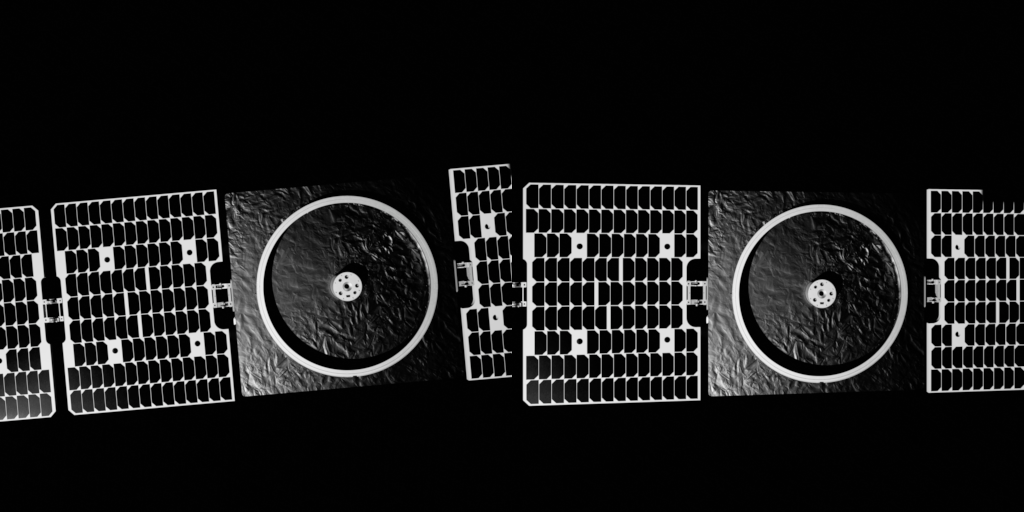
\includegraphics[scale=0.48]{Figures/Chapter1/DatasetExample.png}
    \caption[Sample images from \textit{TASI EROSS IOD Simulated Dataset N°2}]{Sample images from the \textit{TASI EROSS IOD Simulated Dataset N°2}}
    \label{fig:Samples}
\end{figure}
\newpage
The data acquisition has been performed as follow:
\begin{itemize}
    \item \textbf{Non Prepared scenario:} LAR view.
    \item \textbf{Natural Illumination:} Full illumination (sun @45°, 130k lux).
    \item \textbf{Illumination system:} ON (150lm x6 LEDs).
    \item \textbf{Simulated Camera Settings:}
        \begin{itemize}
            \item Shutter speed: 20
            \item ISO: 5
            \item Aperture: 4
            \item FOV: 67.8°
        \end{itemize}
    \item \textbf{Reference System:}
        \begin{itemize}
            \item Left-handed XYZ reference.
            \item Origin [0,0,0]:
            \begin{itemize}
                \item XY: zeroes on the vertical symmetry axis of the Target.
                \item Z: Positive towards contact, zeroed on the lowest contact point of the LAR.
            \end{itemize}
            \item All units are in centimeters (cm).
        \end{itemize}
    \item \textbf{Trajectories:}
        \begin{itemize}
            \item all trajectories follow the same XYZ coordinates.
            \item the rotation is considered with Euler angles as Pitch (around axis x), Yaw (around axis y) and Roll (around axis z), all positive counterclockwise. Trajectories' specifics are reported in table \textbf{\ref{tab:trajectories}}.
            \item Camera pointing XY in [-46, +20].
        \end{itemize}
\end{itemize}

\begin{figure}[th]
    \centering
    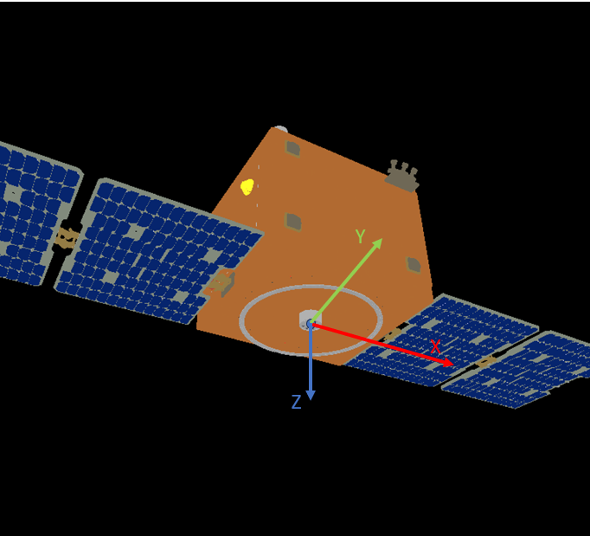
\includegraphics[scale=0.8]{Figures/Chapter1/UPS.png}
    \caption[Model's UPS]{Model's UPS}
    \label{fig:UPS}
\end{figure}

\begin{table}[H]
\caption{Specifics of the simulated training trajectories.}
\label{tab:trajectories}
\centering
\begin{tabular}{l | l l l}
\toprule
Trajectory & Roll(°) & Pitch(°) & Yaw(°)\\
\midrule
TRAY\_1 & 0 & 0 & 0\\
TRAY\_2 & 0 & 0 & -1\\
TRAY\_3 & 0 & 0 & -2\\
TRAY\_4 & 0 & 0 & -3\\
TRAY\_5 & 0 & 0 & -4\\
TRAY\_6 & 0 & 0 & -5\\
TRAY\_7 & 0 & 1 & 0\\
TRAY\_8 & 0 & 2 & 0\\
TRAY\_9 & 0 & 3 & 0\\
TRAY\_10 & 0 & 4 & 0\\
TRAY\_11 & 0 & 5 & 0\\
TRAY\_12 & -1 & 0 & 0\\
TRAY\_13 & -2 & 0 & 0\\
TRAY\_14 & -3 & 0 & 0\\
TRAY\_15 & -4 & 0 & 0\\
TRAY\_16 & -5 & 0 & 0\\
\bottomrule
\end{tabular}
\end{table}

The \textit{TASI EROSS IOD Simulated Dataset N°3} along with the \textit{Less\_Difficult\_Trajectory} and \textit{Difficult\_Trajectory} are used as the test dataset. The \textit{TASI EROSS N°3} is composed of two trajectories, each of which was captured with two different camera positions. Each trajectory has 900 images.\\
The \textit{TRAY\_A} starts with +15° on Yaw and linearly converge toward 0 on contact, while \textit{TRAY\_B}, \textit{Less\_Difficult\ Trajectory} and \textit{Difficult\_Trajectory} present multiple errors on RPY converging toward 0 on contact as well.
\end{comment}
%----------------------------------------------------------------------------------------
%	SECTION 3
%----------------------------------------------------------------------------------------
\section{Thesis structure}
The thesis is structured in further five chapters:
\begin{description}
    \item[Chapter 2] - \textit{Background}:\\ This chapter provides a comprehensive overview of key concepts necessary for the correct understanding of this work, with a focus on monocular camera models, perspective projection, pose estimation, and a general introduction to deep learning models.
    \item[Chapter 3] - \textit{State-of-art}:\\ This chapter delves into monocular pose estimation methods, covering classic approaches like RANSAC and SfM, and exploring modern techniques such as end-to-end learning with networks like PoseNet and Mask R-CNN. The chapter also introduces feature learning, emphasizing CNN-based methods like HRNet for predicting 2D landmark locations. Moreover, some studies about spacecraft pose estimation and their use of deep learning architectures are presented. The chapter also delves into point set alignments, highlighting the widely used and advanced algorithms like Coherent Point Drift (CPD) technique employed in the method for final pose estimation.
    \item[Chapter 4] - \textit{Algorithms and Methods}: \\
    This chapter delves into the methodology's core algorithms and techniques. It outlines the offline architecture, detailing the 2D-3D correspondence process, landmark regression, and the neural network-based landmark mapping. The chapter then presents the online architecture, covering real-time processing and the Coherent Point Drift technique for pose estimation. Implementation challenges and dataset considerations are also discussed, providing a comprehensive overview of the applied methods.
    \item[Chapter 5] - \textit{Implementation and Experiments}:\\
    This chapter presents the tools and technologies employed for the project implementation and the evaluation metrics for pose estimation, Landmark Regression, Landmark Mapping are described. The chapter culminates in the assessment of both training and test datasets, showcasing the method's robustness and generalization across diverse scenarios. Overall, it provides comprehensive exploration of the research's implementation and experimentation phases.
    \item[Chapter 6] - \textit{Discussions and Conclusions}:\\
    The Chapter delves into challenges faced by on-board AI systems in space missions, focusing on verifiability and computational load. It emphasizes the significance of minimizing translation errors for accurate maneuvering in the proposed multi-model configuration. The section explores potential improvements, including enhanced landmark selection and strategies to fortify system robustness.
\end{description}
